\documentclass{standalone}
\usepackage{tikz}
\usetikzlibrary{patterns, positioning}


\begin{document}
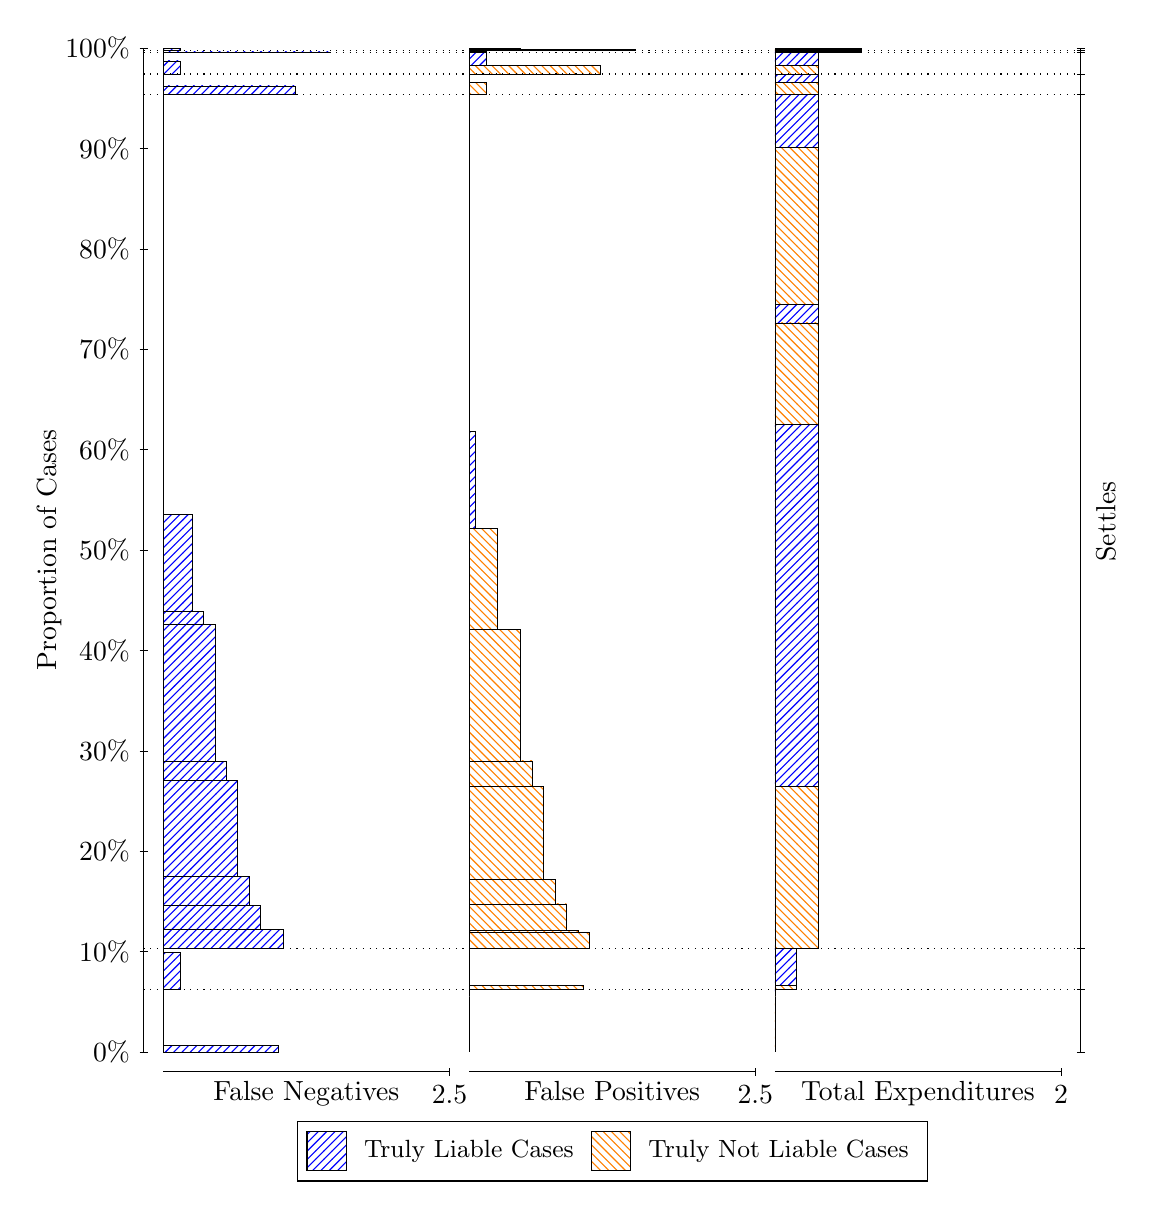
\begin{tikzpicture}
\draw[black, very thin] (1.5,1.75) -- (1.5,14.5);
\node[rotate=90, text=black, anchor=center] at (0.3, 8.125) {Proportion of Cases};
\draw[black, very thin] (1.45,1.75) -- (1.55,1.75);
\node[text=black, anchor=east] at (1.45, 1.75) {0\%};
\draw[black, very thin] (1.45,3.025) -- (1.55,3.025);
\node[text=black, anchor=east] at (1.45, 3.025) {10\%};
\draw[black, very thin] (1.45,4.3) -- (1.55,4.3);
\node[text=black, anchor=east] at (1.45, 4.3) {20\%};
\draw[black, very thin] (1.45,5.575) -- (1.55,5.575);
\node[text=black, anchor=east] at (1.45, 5.575) {30\%};
\draw[black, very thin] (1.45,6.85) -- (1.55,6.85);
\node[text=black, anchor=east] at (1.45, 6.85) {40\%};
\draw[black, very thin] (1.45,8.125) -- (1.55,8.125);
\node[text=black, anchor=east] at (1.45, 8.125) {50\%};
\draw[black, very thin] (1.45,9.4) -- (1.55,9.4);
\node[text=black, anchor=east] at (1.45, 9.4) {60\%};
\draw[black, very thin] (1.45,10.675) -- (1.55,10.675);
\node[text=black, anchor=east] at (1.45, 10.675) {70\%};
\draw[black, very thin] (1.45,11.95) -- (1.55,11.95);
\node[text=black, anchor=east] at (1.45, 11.95) {80\%};
\draw[black, very thin] (1.45,13.225) -- (1.55,13.225);
\node[text=black, anchor=east] at (1.45, 13.225) {90\%};
\draw[black, very thin] (1.45,14.5) -- (1.55,14.5);
\node[text=black, anchor=east] at (1.45, 14.5) {100\%};

\draw[black, very thin] (13.4,1.75) -- (13.4,14.5);
\draw[black, very thin] (13.35,1.75) -- (13.45,1.75);
\node[anchor=west] at (13.35, 1.75) {};
\draw[black, very thin] (13.35,2.5408) -- (13.45,2.5408);
\node[anchor=west] at (13.35, 2.5408) {};
\draw[black, very thin] (13.35,3.068) -- (13.45,3.068);
\node[anchor=west] at (13.35, 3.068) {};
\draw[black, very thin] (13.35,13.91) -- (13.45,13.91);
\node[anchor=west] at (13.35, 13.91) {};
\draw[black, very thin] (13.35,14.17) -- (13.45,14.17);
\node[anchor=west] at (13.35, 14.17) {};
\draw[black, very thin] (13.35,14.443) -- (13.45,14.443);
\node[anchor=west] at (13.35, 14.443) {};
\draw[black, very thin] (13.35,14.47) -- (13.45,14.47);
\node[anchor=west] at (13.35, 14.47) {};
\draw[black, very thin] (13.35,14.5) -- (13.45,14.5);
\node[anchor=west] at (13.35, 14.5) {};

\draw[black, very thin, pattern color=blue, pattern=north east lines] (1.75,1.75) rectangle (3.2033,1.8332);
\draw[black, very thin, pattern color=orange, pattern=north west lines] (1.75,1.8332) rectangle (1.75,2.5408);
\draw[black, very thin, pattern color=blue, pattern=north east lines] (1.75,2.5408) rectangle (1.968,3.0125);
\draw[black, very thin, pattern color=orange, pattern=north west lines] (1.75,3.0125) rectangle (1.75,3.068);
\draw[black, very thin, pattern color=blue, pattern=north east lines] (1.75,3.068) rectangle (3.276,3.305);
\draw[black, very thin, pattern color=blue, pattern=north east lines] (1.75,3.305) rectangle (2.9853,3.6147);
\draw[black, very thin, pattern color=blue, pattern=north east lines] (1.75,3.6147) rectangle (2.84,3.98);
\draw[black, very thin, pattern color=blue, pattern=north east lines] (1.75,3.98) rectangle (2.6947,5.2017);
\draw[black, very thin, pattern color=blue, pattern=north east lines] (1.75,5.2017) rectangle (2.5493,5.4432);
\draw[black, very thin, pattern color=blue, pattern=north east lines] (1.75,5.4432) rectangle (2.404,7.1777);
\draw[black, very thin, pattern color=blue, pattern=north east lines] (1.75,7.1777) rectangle (2.2587,7.3455);
\draw[black, very thin, pattern color=blue, pattern=north east lines] (1.75,7.3455) rectangle (2.1133,8.5802);
\draw[black, very thin, pattern color=orange, pattern=north west lines] (1.75,8.5802) rectangle (1.75,13.91);
\draw[black, very thin, pattern color=blue, pattern=north east lines] (1.75,13.91) rectangle (3.4213,14.02);
\draw[black, very thin, pattern color=orange, pattern=north west lines] (1.75,14.02) rectangle (1.75,14.17);
\draw[black, very thin, pattern color=blue, pattern=north east lines] (1.75,14.17) rectangle (1.968,14.338);
\draw[black, very thin, pattern color=orange, pattern=north west lines] (1.75,14.338) rectangle (1.75,14.443);
\draw[black, very thin, pattern color=blue, pattern=north east lines] (1.75,14.443) rectangle (3.8573,14.452);
\draw[black, very thin, pattern color=orange, pattern=north west lines] (1.75,14.452) rectangle (1.75,14.47);
\draw[black, very thin, pattern color=blue, pattern=north east lines] (1.75,14.47) rectangle (1.968,14.491);
\draw[black, very thin, pattern color=orange, pattern=north west lines] (1.75,14.491) rectangle (1.75,14.5);
\draw[black, very thin, pattern color=orange, pattern=north west lines] (5.6333,1.75) rectangle (5.6333,2.4576);
\draw[black, very thin, pattern color=blue, pattern=north east lines] (5.6333,2.4576) rectangle (5.6333,2.5408);
\draw[black, very thin, pattern color=orange, pattern=north west lines] (5.6333,2.5408) rectangle (7.0867,2.5963);
\draw[black, very thin, pattern color=blue, pattern=north east lines] (5.6333,2.5963) rectangle (5.6333,3.068);
\draw[black, very thin, pattern color=orange, pattern=north west lines] (5.6333,3.068) rectangle (7.1593,3.2677);
\draw[black, very thin, pattern color=orange, pattern=north west lines] (5.6333,3.2677) rectangle (7.014,3.2942);
\draw[black, very thin, pattern color=orange, pattern=north west lines] (5.6333,3.2942) rectangle (6.8687,3.6313);
\draw[black, very thin, pattern color=orange, pattern=north west lines] (5.6333,3.6313) rectangle (6.7233,3.9377);
\draw[black, very thin, pattern color=orange, pattern=north west lines] (5.6333,3.9377) rectangle (6.578,5.1221);
\draw[black, very thin, pattern color=orange, pattern=north west lines] (5.6333,5.1221) rectangle (6.4327,5.4472);
\draw[black, very thin, pattern color=orange, pattern=north west lines] (5.6333,5.4472) rectangle (6.2873,7.1121);
\draw[black, very thin, pattern color=orange, pattern=north west lines] (5.6333,7.1121) rectangle (5.9967,8.3977);
\draw[black, very thin, pattern color=blue, pattern=north east lines] (5.6333,8.3977) rectangle (5.706,9.6325);
\draw[black, very thin, pattern color=blue, pattern=north east lines] (5.6333,9.6325) rectangle (5.6333,13.91);
\draw[black, very thin, pattern color=orange, pattern=north west lines] (5.6333,13.91) rectangle (5.8513,14.06);
\draw[black, very thin, pattern color=blue, pattern=north east lines] (5.6333,14.06) rectangle (5.6333,14.17);
\draw[black, very thin, pattern color=orange, pattern=north west lines] (5.6333,14.17) rectangle (7.3047,14.275);
\draw[black, very thin, pattern color=blue, pattern=north east lines] (5.6333,14.275) rectangle (5.8513,14.443);
\draw[black, very thin, pattern color=orange, pattern=north west lines] (5.6333,14.443) rectangle (5.8513,14.461);
\draw[black, very thin, pattern color=blue, pattern=north east lines] (5.6333,14.461) rectangle (5.6333,14.47);
\draw[black, very thin, pattern color=orange, pattern=north west lines] (5.6333,14.47) rectangle (7.7407,14.479);
\draw[black, very thin, pattern color=blue, pattern=north east lines] (5.6333,14.479) rectangle (6.2873,14.5);
\draw[black, very thin, pattern color=orange, pattern=north west lines] (9.5167,1.75) rectangle (9.5167,2.4576);
\draw[black, very thin, pattern color=blue, pattern=north east lines] (9.5167,2.4576) rectangle (9.5167,2.5408);
\draw[black, very thin, pattern color=orange, pattern=north west lines] (9.5167,2.5408) rectangle (9.7892,2.5963);
\draw[black, very thin, pattern color=blue, pattern=north east lines] (9.5167,2.5963) rectangle (9.7892,3.068);
\draw[black, very thin, pattern color=orange, pattern=north west lines] (9.5167,3.068) rectangle (10.062,5.1221);
\draw[black, very thin, pattern color=blue, pattern=north east lines] (9.5167,5.1221) rectangle (10.062,9.7223);
\draw[black, very thin, pattern color=orange, pattern=north west lines] (9.5167,9.7223) rectangle (10.062,11.008);
\draw[black, very thin, pattern color=blue, pattern=north east lines] (9.5167,11.008) rectangle (10.062,11.245);
\draw[black, very thin, pattern color=orange, pattern=north west lines] (9.5167,11.245) rectangle (10.062,13.235);
\draw[black, very thin, pattern color=blue, pattern=north east lines] (9.5167,13.235) rectangle (10.062,13.91);
\draw[black, very thin, pattern color=orange, pattern=north west lines] (9.5167,13.91) rectangle (10.062,14.06);
\draw[black, very thin, pattern color=blue, pattern=north east lines] (9.5167,14.06) rectangle (10.062,14.17);
\draw[black, very thin, pattern color=orange, pattern=north west lines] (9.5167,14.17) rectangle (10.062,14.275);
\draw[black, very thin, pattern color=blue, pattern=north east lines] (9.5167,14.275) rectangle (10.062,14.443);
\draw[black, very thin, pattern color=orange, pattern=north west lines] (9.5167,14.443) rectangle (10.607,14.461);
\draw[black, very thin, pattern color=blue, pattern=north east lines] (9.5167,14.461) rectangle (10.607,14.47);
\draw[black, very thin, pattern color=orange, pattern=north west lines] (9.5167,14.47) rectangle (10.607,14.479);
\draw[black, very thin, pattern color=blue, pattern=north east lines] (9.5167,14.479) rectangle (10.607,14.5);
\draw[black, dotted] (1.5,2.5408) -- (13.4,2.5408);
\draw[black, dotted] (1.5,3.068) -- (13.4,3.068);
\draw[black, dotted] (1.5,13.91) -- (13.4,13.91);
\draw[black, dotted] (1.5,14.17) -- (13.4,14.17);
\draw[black, dotted] (1.5,14.443) -- (13.4,14.443);
\draw[black, dotted] (1.5,14.47) -- (13.4,14.47);
\draw[black, very thin] (1.75,1.5) -- (5.3833,1.5);
\node[text=black, anchor=north] at (3.5667, 1.5) {False Negatives};
\draw[black, very thin] (5.3833,1.45) -- (5.3833,1.55);
\node[text=black, anchor=north] at (5.3833, 1.45) {2.5};

\draw[black, very thin] (5.6333,1.5) -- (9.2667,1.5);
\node[text=black, anchor=north] at (7.45, 1.5) {False Positives};
\draw[black, very thin] (9.2667,1.45) -- (9.2667,1.55);
\node[text=black, anchor=north] at (9.2667, 1.45) {2.5};

\draw[black, very thin] (9.5167,1.5) -- (13.15,1.5);
\node[text=black, anchor=north] at (11.333, 1.5) {Total Expenditures};
\draw[black, very thin] (13.15,1.45) -- (13.15,1.55);
\node[text=black, anchor=north] at (13.15, 1.45) {2};



\node[text=black, centered, rotate=90] at (13.72, 8.489) {Settles};





\draw (7.449999999999999,1.5) node[draw=none] (baseCoordinate) {};
\begin{scope}[align=center]
        \matrix[scale=0.5, draw=black, below=0.5cm of baseCoordinate, nodes={draw}, column sep=0.1cm]{
            \node[rectangle, draw, minimum width=0.5cm, minimum height=0.5cm, pattern color=blue, pattern=north east lines] {}; &
            \node[draw=none, font=\small, text=black] (B) {Truly Liable Cases}; &
            \node[rectangle, draw, minimum width=0.5cm, minimum height=0.5cm, pattern color=orange, pattern=north west lines] {}; &
            \node[draw=none, font=\small, text=black] (B) {Truly Not Liable Cases}; \\
            };
\end{scope}

\end{tikzpicture}
\end{document}